\documentclass[10pt]{article}
\usepackage[polish]{babel}
\usepackage[utf8]{inputenc}
\usepackage[T1]{fontenc}
\usepackage{amsmath}
\usepackage{amsfonts}
\usepackage{amssymb}
\usepackage[version=4]{mhchem}
\usepackage{stmaryrd}
\usepackage{graphicx}
\usepackage[export]{adjustbox}
\graphicspath{ {./images/} }

\title{LIGA MATEMATYCZNA im. Zdzisława Matuskiego \\
 PAŹDZIERNIK 2016 \\
 GIMNAZJUM }

\author{}
\date{}


\begin{document}
\maketitle
\section*{ZADANIE 1.}
W okrąg o promieniu o długości 10 wpisano prostokąt \(A B C D\). Następnie na tym okręgu wybrano dowolny punkt \(E\). Oblicz sumę kwadratów odległości punktu \(E\) od wierzchołków prostokąta, czyli \(|E A|^{2}+|E B|^{2}+|E C|^{2}+|E D|^{2}\).

\section*{ZADANIE 2.}
Ile jest dodatnich liczb całkowitych, których największy dzielnik właściwy (to znaczy dzielnik różny od 1 i od danej liczby) jest równy 91 ?

\section*{ZADANIE 3.}
Ania ma 36 karteczek. Pomalowała je używając trzech kolorów: zielonego, czerwonego i niebieskiego. Niektóre karteczki są pomalowane tylko jednym kolorem, inne dwoma, a pozostałe pięć karteczek wszystkimi trzema kolorami. Zielonej kredki użyła do pokolorowania 25 karteczek, czerwonej do 28, a niebieskiej do 20 karteczek. Ile karteczek Ania pomalowała jednym kolorem?

\section*{ZADANIE 4.}
Operacją nazywamy przyporządkowanie trójce liczb \((a, b, c)\) nowej trójki \((b+c, a+c, a+b)\). Początkową trójką jest \((1,3,5)\). Po wykonaniu 2016 takich operacji na otrzymywanych trójkach liczb uzyskano \((x, y, z)\). Oblicz różnicę \(x-y\).

\section*{ZADANIE 5.}
Dany jest prostokąt \(A B C D\), w którym \(|A B|=20,|B C|=10\). Punkty \(W\) i \(K\) leżą na zewnątrz tego prostokąta oraz \(|W A|=|K C|=12\) oraz \(|W B|=|K D|=16\). Oblicz długość odcinka WK.\\
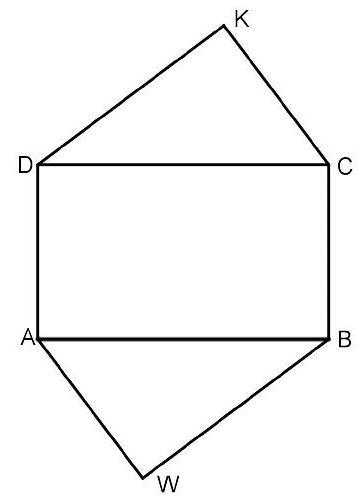
\includegraphics[max width=\textwidth, center]{2024_11_21_d7e50f3a037c14077f6eg-1}


\end{document}